\documentclass[tikz,border=5pt]{standalone}
\usepackage{tikz}
\usepackage{tikzscale}
\usetikzlibrary{positioning}
\usetikzlibrary{positioning,arrows.meta}
\begin{document}
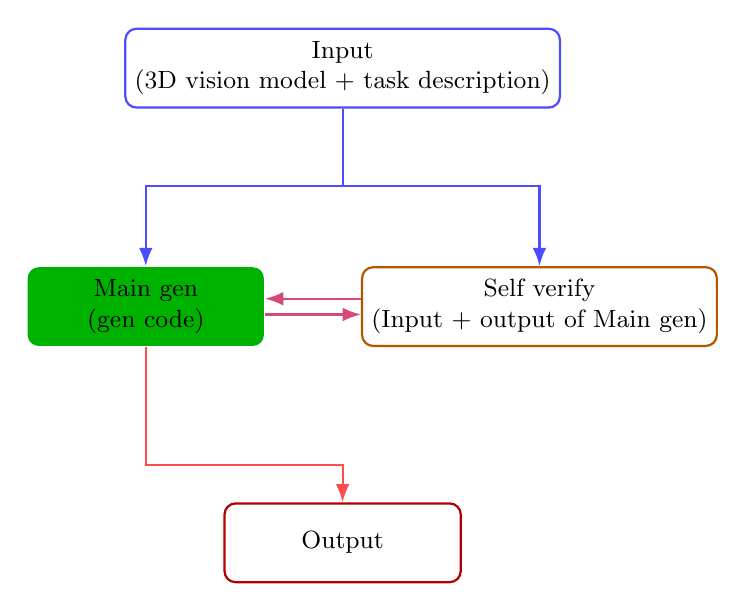
\begin{tikzpicture}[node distance=2cm and 2.5cm]
\tikzset{
    inputStyle/.style={rectangle, draw=blue!70, thick, rounded corners, minimum width=3cm, minimum height=1cm, align=center, font=\small},
    mainStyle/.style={rectangle, fill=green!70!black, thick, rounded corners, minimum width=3cm, minimum height=1cm, align=center, font=\small},
    verifyStyle/.style={rectangle, draw=orange!70!black, thick, rounded corners, minimum width=3cm, minimum height=1cm, align=center, font=\small},
    outputStyle/.style={rectangle, draw=red!70!black, thick, rounded corners, minimum width=3cm, minimum height=1cm, align=center, font=\small},
    inputArrow/.style={-Latex, thick, blue!70},
    communicationArrow/.style={-Latex, thick, purple!70},
    outputArrow/.style={-Latex, thick, red!70}
}


\node[inputStyle] (input) {Input\\(3D vision model + task description)};

\node[mainStyle, below=2cm of input, xshift=-2.5cm] (main) {Main gen\\(gen code)};
\node[verifyStyle, below=2cm of input, xshift=2.5cm] (verify) {Self verify\\(Input + output of Main gen)};

\node[outputStyle, below=5cm of input] (output) {Output};


\draw[inputArrow] (input.south) -- (0,-1.5) -| (main.north);
\draw[inputArrow] (input.south) -- (0,-1.5) -| (verify.north);



\draw[communicationArrow] ([yshift=-0.1cm]main.east) -- ++(1,0) |- ([yshift=-0.1cm]verify.west);


\draw[communicationArrow] ([yshift=0.1cm]verify.west) -- ++(-1,0) |- ([yshift=0.1cm]main.east);

\draw[outputArrow] (main.south) -- ++(0,-1.5) -| (output.north);


\end{tikzpicture}

\end{document}